\section{Systems of Differential Equations}

Just like in conventional algebra problems, we can have systems of differential equations. A solution of a system of two differential equations is a pair of functions $x(t)$ and $y(t)$ that satisfy both equations.

The resulting equation can also be though of as a three dimensional solution in the form $(x(t), y(t)) = t$.

If one or more functions are dependent on other functions, then we call them coupled. Otherwise we call them decoupled.
\[
\begin{aligned}
\text{Coupled}
\begin{cases}
y\prime = xy\\
x\prime = yx
\end{cases}\\
\text{Decoupled}
\begin{cases}
y\prime = yt\\
x\prime = xt
\end{cases}
\end{aligned}
\]

    \subsection{Autonomous First Order System}
    Autonomous systems are not dependent on $t$, so we can treat them a little differently. For these equations we can use a phase plane, vector field, and the trajectory of the solution.

    The functions $x(t)$ and $y(t)$ can give us a parametric curve. This means that at any given point on the curve, we also have a tangent vector given by $\frac{dy}{dt}$ and$\frac{dx}{dt}$.

    Every solution of a system we call a state of the system, and the collection of all the trajectories and states is called a phase portrait.

    An equilibrium point for this two dimensional system is an $(x,y)$ point where
    \[
    \frac{dy}{dt} = 0 = \frac{dx}{dt}
    \]

    \subsection{Graphical Methods for Solving}
    Sketching is a pain in the ass\dots Therefore there are a couple tricks that we can use to make our lives easier.

    We can use nullclines to more easily draw the solutions. Nullclines are an adaptation of previously mentioned isoclines \eqref{sec:visde}. A V nullcline is an isocline of vertical slopes where $x\prime = 0$. An H nullcline is an isocline of horizontal slopes where $y\prime = 0$. Equilibria occurs at the point where these two nullclines intersect.

    Note, when existence and uniqueness hold for an autonomous system, phase plane trajectories never cross.

    \begin{figure}[ht]\label{fig:visrep}
    \centering
        \begin{subfigure}[b]{0.4\textwidth}
            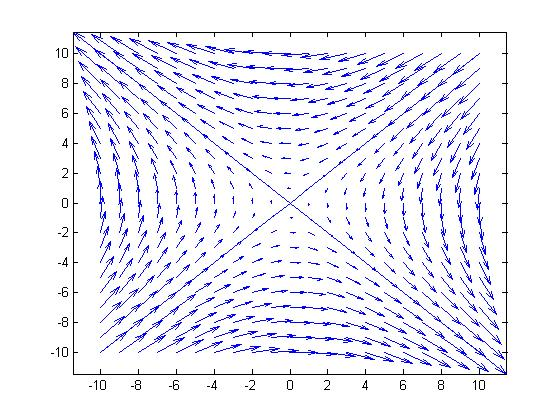
\includegraphics[scale=0.25]{./img/vectorfield.png}
            \caption{Vector Field}
        \end{subfigure}
        \begin{subfigure}[b]{0.4\textwidth}
            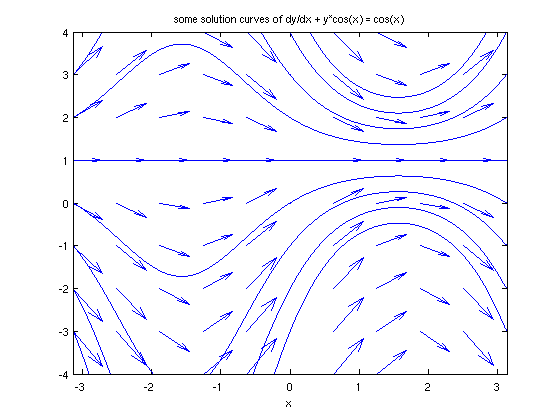
\includegraphics[scale=0.25]{./img/solutioncurves.png}
            \caption{Solution Curves}
        \end{subfigure}
    \caption{Visual Representations}
    \end{figure}

    \subsection{Quick Sketching Outline for Phase Portraits}
    \begin{enumerate}
    \item Nullclines and Equilibria
        \begin{itemize}
        \item Where $x\prime = 0$, slopes are vertical.
        \item Where $y\prime = 0$, slopes are horizontal.
        \item Where $x\prime = y\prime = 0$, we have equilibria.
        \end{itemize}
    \item Left-Right Directions
        \begin{itemize}
        \item Where $x\prime$ is positive, arrows point right.
        \item Where $x\prime$ is negative, arrows point left.
        \end{itemize}
    \item Up-Down Directions
        \begin{itemize}
        \item Where $y\prime$ is positive, arrows point up.
        \item Where $y\prime$ is negative, arrows point down.
        \end{itemize}
    \item Check Uniqueness\\
    Where phase plane trajectories do not cross, we have uniqueness.
    \end{enumerate}

    \subsection{Applications of Systems of Differential Equations}
        \subsubsection{Predator-Prey Assumptions}
        In the absence of foxes, the rabbit population will grow with the Malthusian Growth Law:
        \[
        \frac{dR}{dt} = a_R R, a_R > 0
        \]
        In the absence of rabbits, the fox population will die off according to the law:
        \[
        \frac{dF}{dtt} = -a_F F, a_F > 0
        \]
        When both foxes and rabbits are present, the number of interactions is $\propto$ the product of the population sizes, with inverse behavior. Thus we can get the Lotka-Volterra Equations for the predator prey model:

        \begin{equation}\label{eq:LVeq}
        \begin{cases}
        \frac{dR}{dt} = a_R R - c_R RF\\
        \frac{dF}{dt} = -a_F F - c_F RF
        \end{cases}
        \end{equation}

\section{Matrices}
    Using matrices enables us to do more complex operations on systems of equations, as well as other numbers and functions.

    \subsection{Definitions}
    A matrix is a rectangular array of elements arranged in rows and columns.

    \begin{equation}\label{eq:matrixdef}
    \mathbf{A} =
    \left[ \begin{matrix}
        a_1 & a_2 & a_3 & \cdots & a_n\\
        b_1 & b_2 & b_j & \cdots & b_n\\
        c_1 & c_2 & c_3 & \cdots & c_n\\
        \vdots & \vdots & \vdots & \ddots & \vdots\\
        m_1 & m_2 & m_3 & \cdots & m_n\\
    \end{matrix} \right]
    \end{equation}\myequations{Mathematical Definition of a Matrix}

    We can also describe these matrices by saying it has order $m \times n$ where $m$ and $n$ are the row and column sizes respectively. Two matrices are equal if they have the same $m$ and $n$ and the values contained are equal. We can also have matrices with orders $m \times 1$ or $n \times 1$ which are called column and row vectors.

    If all entries are 0, we call it a zero matrix; however if all entries but the diagonal are zero, this is called an diagonal matrix. These diagonal number are called diagonal elements. A special diagonal matrix is the identity matrix, which is formed when the diagonal elements are ones.

    \begin{equation}\label{eq:id_matrix}
        \left[ \begin{array}{cccc}
        1 & 0 & \cdots & 0\\
        0 & 1 & \cdots & 0\\
        \vdots & \vdots & 1 & \vdots\\
        0 & 0 & \cdots & 1\\
        \end{array} \right]
    \end{equation}

    \subsection{Addition and Multiplication}
    Most of the basic mathematical operations also apply to matrices. When adding two matrices, just add the components, when multiplying by a scalar, multiply each component by the scalar.

    Multiplication of two matrices is a little different however. When multiplying two matrices labeled $\mathbf{A}$ and $\mathbf{B}$ the steps are represented as follows.

    \begin{center}
        \textit{Each new element in the matrix is a result of the dot product between the corresponding row and column matrices.}
    \end{center}
    \begin{equation}\label{eq:matrixmultiplication}
    \begin{aligned}
        \mathbf{A}=
        \left[\begin{matrix}
        A_{11} & A_{12} & \cdots & A_{1m} \\
        A_{21} & A_{22} & \cdots & A_{2m} \\
        \vdots & \vdots & \ddots & \vdots \\
        A_{n1} & A_{n2} & \cdots & A_{nm} \\
        \end{matrix}\right]\\
        \quad\mathbf{B}=
        \left[\begin{matrix}
        B_{11} & B_{12} & \cdots & B_{1p} \\
        B_{21} & B_{22} & \cdots & B_{2p} \\
        \vdots & \vdots & \ddots & \vdots \\
        B_{m1} & B_{m2} & \cdots & B_{mp} \\
        \end{matrix}\right]\\
        \mathbf{A}\mathbf{B}=
        \left[\begin{matrix}
        A_1 \cdot B_1 & A_2 \cdot B_1 & \cdots & A_3 \cdot B_1 \\
        A_2 \cdot B_1 & A_2 \cdot B_2 & \cdots & A_2 \cdot B_3 \\
        \vdots & \vdots & \ddots & \vdots \\
        A_m \cdot B_1 & A_m \cdot B_2 & \cdots & A_m \cdot B_n \\
        \end{matrix}\right]
    \end{aligned}
    \end{equation}\myequations{Mathematical Matrix Multiplication}

    \subsection{Matrix Transposition}
    We can flip a matrix diagonally so that its columns become rows and its rows become columns. We call this the transpose of the matrix, written $\mathbf{A}^T$.

        \subsubsection{Example}
        \[
        \text{If } \mathbf{A} = \left[ \begin{array}{cc}
            1 & 2\\
            3 & 4\\
            5 & 6\\
        \end{array} \right] \text{ Then } \mathbf{A}^T
        \left[ \begin{array}{ccc}
            1 & 3 & 5\\
            2 & 4 & 6\\
        \end{array} \right]
        \]

        \subsubsection{Properties}
        \begin{itemize}
            \item ${(\ma^T)}^T = \ma$
            \item ${(\ma + \mb)}^T = \ma^T + \mb^T$
            \item ${(k \ma)}^T = k\ma^T$ for any scalar $k$.
            \item ${(\ma \mb)}^T = \ma^T \mb^T$
        \end{itemize}

    \subsection{Vectors as Special Matrices}
    For a given vector in $\mathbb{R}^n$, we can write

    \[
        \vec{x} =
        \left[\begin{matrix}
        x_1\\
        x_2\\
        \vdots\\
        x_n
        \end{matrix}\right] \text{ and }
        \vec{y} =
        \left[\begin{matrix}
        y_1\\
        y_2\\
        \vdots\\
        y_n
        \end{matrix}\right]
    \]
    We can also find the dot product of two matrices represented in this form using rules for matrix multiplication. Two vectors are orthogonal if their dot product is zero (See my Calculus III Notes\footnote{\attachfile{./img/CalcIIINotes.pdf}{Calc III Notes}\label{doc:calcIII}\myequations{Calc III Notes} }, section 2, for more information).

    The absolute value of one of these vectors is equal to the matrix dotted with itself and square-rooted.

    \begin{equation}\label{eq:matrix_abs_val}
        ||\vec{v}|| \equiv \sqrt{\vec{v} \cdot \vec{v} }
    \end{equation}\myequations{Absolute Value of a Vector Matrix}

\section{Matrices and Systems of Linear Equations}
Up until this point we've been solving systems of linear equations through fiddling with them (solving for different variables, etc.) until we get an answer. Using matrices we can solve them a lot more effectively. Not only that, but any process we use will turn the matrix into an equivalent system of equations, i.e., one that has the same solutions.

We can have systems of linear equations represented in matrices, and if all equations are equal to zero, the system is homogeneous. The solution is defined as the point in $\mathbb{R}^n$ whose coordinates solve the system of equations.

We have a couple of methods to solve systems of linear equations when they are in matrix form, but first we need to define a couple different terms and operations.

    \subsection{Augmented Matrix}
    An augmented matrix is where two different matrices are combined to form a new matrix.

    \begin{equation}\label{eq:augmented_matrix}
    \begin{aligned}
        \mathbf{[A|b]}=
        \left[\begin{array}{cccc|c}
        A_{11} & A_{12} & \cdots & A_{1m} & b_1\\
        A_{21} & A_{22} & \cdots & A_{2m} & b_2\\
        \vdots & \vdots & \ddots & \vdots & \vdots\\
        A_{n1} & A_{n2} & \cdots & A_{nm} & b_n\\
        \end{array}\right]\\
    \end{aligned}
    \end{equation}\myequations{Augmented Matrix}

    This is usually used to show the coefficients of the variables in a system of equations as well as the constants they are equal to.

    \subsection{Elementary Row Operations}
    We have a couple of different options to manipulate augmented matrices, which are as follows.

    \begin{itemize}
        \item Interchange row $i$ and $i$
            \[ R^*_i = R_j, R^*_j = R_i \]
        \item Multiply row $i$ by a constant.
            \[ R^*_i = cR_i \]
        \item Leaving $j$ untouched, add to $i$ a constant times $j$.
            \[ R^*_i = R_i + cR_j \]
    \end{itemize}

    These are handy when dealing with matrices and trying to obtain Reduced Row Echelon Form \eqref{sec:RREF}.

    \subsection{Reduced Row Echelon Form}\label{sec:RREF}
    When dealing with systems of linear equations in augmented matrix form we need to get it to a solution, which can be found with Reduced Row Echelon Form (RREF). This form looks similar to the following.

    \begin{equation}\label{eq:rref}
    \begin{aligned}
        \mathbf{[A|b]}=
        \left[\begin{array}{ccc|c}
        1 & 0 & 0 & b_1\\
        0 & 1 & 0 & b_2\\
        0 & 0 & 1 & b_3\\
        \end{array}\right]\\
    \end{aligned}
    \end{equation}\myequations{Reduced Row Echelon Form}

    This can be characterized by the following:

    \begin{itemize}
        \item $0$ rows are at the bottom.
        \item Leftmost non-zero entry is $1$, also called the pivot (or leading 1).
        \item Each pivot is further to the right than the one above.
        \item Each pivot is the only non-zero entry in its column.
    \end{itemize}

    A less complete process gives us row echelon form, which allows for nonzero entries are allowed above the pivot.

    \subsection{Gauss Jordan Reduction}
    This procedure will let us solve any given matrix/linear system. The steps are as follows.

    \begin{enumerate}
        \item Given a system $A\vec{x} = \vec{b}$
        \item Form augmented matrix $[A|b]$
        \item Transform to RREF \eqref{sec:RREF} using elementary row operations.
        \item The linear matrix formed by this process has the same solutions as the initial system, however it is much easier to solve.
    \end{enumerate}

    \subsection{Existence and Uniqueness}
    If the RREF has a row that looks like:
    \[
        [0, 0, 0, \cdots, 0 | k]
    \]
    where $k$ is a non-zero constant, then the system has no solutions. We call this inconsistent.

    If the system has one or more solutions, we call it consistent.

    In order to be unique, the system needs to be consistent.
        \begin{itemize}
            \item If every column is a pivot, the there is only one solution (unique solution).
            \item Else If most columns are pivots, there are multiple solutions (possibly infinite).
            \item Else the system is inconsistent.
        \end{itemize}

    \subsection{Superposition, Nonhomogeneous Principle, and RREF}
    For any nonhomogeneous linear system $\mathbf{A}\vec{x} = \vec{b}$, we can write the solutions as:
    \[
        \vec{x} = \vec{x}_h + \vec{x}_p
    \]
    Where $\vec{x}_h$ represents vectors in the set of homogeneous solutions, and $\vec{x}_p$ is a particular solution to the original equation.

    We can use RREF to find $\vec{x}_p$, and then, using the same RREF with $\vec{b}$ replaced by $\vec{0}$, find $\vec{x}_h$.

    The rank of a matrix $r$ equals the number of pivot columns in the RREF. If $r$ equals the number of variables, there is a unique solution. Otherwise if there is less, then it is not unique.

    \subsection{Inverse of a Matrix}
    When given a system of equations like:
    \[
        \begin{cases}
            x + y = 1\\
            4x + 5y = 6
        \end{cases}
    \]
    we can rewrite it in the form:
    \[
        \left[\begin{array}{cc}
        1 & 1\\
        4 & 5
        \end{array}\right]
        \left[\begin{array}{c}
            x\\
            y
        \end{array}\right] =
        \left[\begin{array}{c}
            1\\
            6
        \end{array}\right]
    \]
    For this sort of matrix, we can find the inverse which is defined as the matrix that, when multiplied with the original, equals an Identity Matrix. In other words:
    \[ A^{-1}A = AA^{-1} = I \]

        \subsubsection{Properties}
        \begin{itemize}
        \item ${( A^{-1})}^{-1} = A$
        \item $A$ and $B$ are invertible matrices of the same order if $\left(AB\right) = A^{-1}B^{-1}$
        \item If $A$ is invertible, then so is $A^T$ and $\left(A^{-1}\right)^T = \left(A^T\right)^{-1}$
        \end{itemize}

        \subsubsection{Inverse Matrix by RREF}
        For an $n\times n$ matrix $A$, the following procedure either produces $A^{-1}$, or proves that it's impossible.

        \begin{enumerate}
        \item Form the $n \times 2n$ matrix $M=\left[A|I\right]$
        \item Transform $M$ into its RREF, $R$.
        \item If the first $n$ columns produce an Identity Matrix, then the last $n$ are its inverse. Otherwise $A$ is not invertible.
        \end{enumerate}

    \subsection{Invertibility and Solutions}
    The matrix vector equation $A\mathbf{x} = b$ where $A$ is an $n \times n$ matrix has:
        \begin{itemize}
        \item A unique solution $x=A^{-1} b$ if and only if $A$ is invertible.
        \item Either no solutions or infinitely many solutions if $A$ is not invertible.
        \end{itemize}

    For the homogeneous equation $A \mathbf{x} = 0$, there is always one solution, $x=0$ called the trivial solution.

    Let $\ma$ be an $n \times n$ matrix. The following statements apply.
    \begin{itemize}
        \item $\ma$ is an invertible matrix.
        \item $\ma^T$ is an invertible matrix.
        \item $\ma$ is row equivalent to $I_n$.
        \item $\ma$ has $n$ pivot columns.
        \item The equation $\ma \vec{x} = \vec{0}$ has only the trivial solution, $\vec{x}=\vec{0}$.
        \item The equation $\ma \vec{x} = \vec{0}$ has a unique solution for every $\vec{b}$ in $\mathbb{R}^n$.
    \end{itemize}

    \subsection{Determinants and Cramer's Rule}
    The determinant of a square matrix is a scalar number associated with that matrix. These are very important.

        \subsubsection{$2 \times 2$ Matrix}\label{subsubsec:22mat}
        To find the determinant of a $2 \times 2$ matrix, the determinant is the diagonal products subtracted. This process is demonstrated below.

        \begin{equation}\label{eq:22det}
        \begin{aligned}
            A =
            \left[\begin{array}{cc}
                a_{11} & a_{12}\\
                a_{21} & a_{22}
            \end{array}\right]\\
            \left| A \right| = a_{22} \cdot a_{11} - a_{12} \cdot a_{21}
        \end{aligned}
        \end{equation}\myequations{Determinant of a $2 \times 2$ Matrix}

        \subsubsection{Definitions}
        Every element of a $n \times n$ matrix has an associated minor and cofactor.

        \begin{itemize}
        \item Minor $\to$ A $(n - 1) \times (n - 1)$ matrix obtained by deleting the $i$th row and $j$th column of $A$.
        \item Cofactor $\to$ The scalar $C_{ij} = (C - 1)^{i+j} \left| M_{ij} \right|$
        \end{itemize}

        \subsubsection{Recursive Method of an $n \times n$ matrix $A$}
        We can now determine a recursive method for any $n \times n$ matrix.

        Using the definitions declared above, we use the recursive method that follows.

        \begin{equation}\label{eq:detrec}
        \left| A \right| = \sum_{j=1}^n a_{ij} C_{ij}
        \end{equation}\myequations{Recursive Method for Obtaining the Determinant of an $n \times n$ Matrix}

        Find $j$ and then finish with the rules for the $2 \times 2$ matrix defined above in \eqref{subsubsec:22mat}.

        \subsubsection{Row Operations and Determinants}
        Let $A$ be square.

        \begin{itemize}
        \item If two rows of $A$ are exchanged to get $B$, then $|B| = -|A|$.
        \item If one row of $A$ is multiplied by a constant $c$, and then added to another row to get $B$, then $|A| = |B|$.
        \item If one row of $A$ is multiplied by a constant $c$, then $|B| = c|A|$.
        \item If $|A| = 0$, $A$ is called singular.
        \end{itemize}

        For an $n \times n$ $A$ and $B$, the determinant $|AB|$ is given by $|A||B|$.

        \subsubsection{Properties of Determinants}
        \begin{itemize}
        \item If two rows of $\ma$ are interchanged to equal $\mb$, then
            \[ | \mb | = - | \ma | \]
        \item If one row of $\ma$ is multiplied by a constant $k$, and then added to another row to produce matrix $\mb$, then
            \[ | \mb | = | \ma | \]
        \item If one row of $\ma$ is multiplied by $k$ to produce matrix $\mb$, then
            \[ | \mb | = k | \ma | \]
        \item If $|AB| = 0$, then either $|A|$ or $|B|$ must be zero.
        \item $|A^T| = A$
        \item If $| \ma | \neq 0$, then $| \ma^{-1} | = \frac{1}{|\ma |}$.
        \item If $A$ is an upper or lower triangle matrix\footnote{A triangle matrix is one where either the lower or upper half is zero, e.g. $\left[\begin{array}{cccc}1 & 0 & 0 & 0\\1 & 1 & 0 & 0\\1 & 1 & 1 & 0\\1 & 1 & 1 & 1\end{array}\right]$.}, then the determinant is the product of the diagonals.
        \item If one row or column consists of only zeros, then $|A| = 0$.
        \item If two rows or columns are equal, then $|A|=0$.
        \item $A$ is invertible.
        \item $A^T$ is also invertible.
        \item $A$ has $n$ pivot columns.
        \item $|A| \neq 0$
        \item If $|A| = 0$ it is called singular, otherwise it is nonsingular.
        \end{itemize}

        \subsubsection{Cramer's Rule}
        For the $n \times n$ matrix $A$ with $|A| \neq 0$, denote by $A_i$ the matrix obtained from $A$ by replacing its $i$th column with the column vector $\mathbf{b}$. Then the $i$th component of the solution of the system is given by:

        \begin{equation}\label{eq:cramer}
            x_i = \frac{|A_i|}{|A|}
        \end{equation}\myequations{Cramer's Rule}


\section{Vector Spaces and Subspaces}
A vector space $\mathcal{V}$ is a non-empty collection of elements that we call vectors, for which we can define the operation of vector addition and scalar multiplication:
    \begin{enumerate}
    \item Addition: $\vec{x} + \vec{y}$
    \item Scalars: $c \vec{x}$ where $c$ is a constant.
    \end{enumerate}
that satisfy the following properties:
    \begin{enumerate}
    \item $\vec{x} + \vec{y} \in \mathcal{V}$
    \item $c \vec{x} \in \mathcal{V}$
    \end{enumerate}

which can be condensed into a single equation:
\[
    c\vec{x} + d\vec{y} \in \mathcal{V}
\]
which is called closure under linear combinations.

    \subsection{Properties}
    We have the properties from before, as well as new ones.

    \begin{enumerate}
    \item $\vec{x} + \vec{y} \in \mathcal{V} \leftarrow $ Addition
    \item $c \vec{x} \in \mathcal{V} \leftarrow $ Scalar Multiplication
    \item $\vec{x} + \vec{0} = \vec{x} \leftarrow $ Zero Element
    \item $\vec{x} + (-\vec{x}) = (-\vec{x}) + \vec{x} = \vec{0} \leftarrow $ Additive Inverse
    \item $(\vec{x} + \vec{y}) + \vec{z} = \vec{x} + (\vec{y} + \vec{z}) \leftarrow$ Associative Property
    \item $\vec{x} + \vec{y} = \vec{y} + \vec{x} \leftarrow $ Commutativity
    \item $1 \cdot \vec{x} = \vec{x} \leftarrow$ Identity
    \item $c (\vec{x} + \vec{y}) = c\vec{x} + c\vec{y} \leftarrow $ Distributive Property
    \item $(c + d) \vec{x} = c\vec{x} + d\vec{x} \leftarrow $ Distributive Property
    \item $c(d\vec{x}) = (cd)\vec{x} \leftarrow $ Associativity
    \end{enumerate}

    \subsection{Vector Function Space}
    A vector function space is just a unique vector space where the elements of the space are functions.

    Note, the solutions to linear and homogeneous differential equations form vector spaces.

        \subsubsection{Closure under Linear Combination}
        \begin{equation}\label{eq:funcspace_closure}
            c \vec{x} + d \vec{y} \in \mathbb{V} \text{ whenever } \vec{x}, \vec{y} \in \mathbb{V} \text{ and } c, d \in \mathbb{R}
        \end{equation}\myequations{Vector Function Space Closure Under Linear Combinations}

        \subsubsection{Prominent Vector Function Spaces}
        \begin{itemize}
            \item $\mathbb{R}^2 \to$ The space of all ordered pairs.
            \item $\mathbb{R}^3 \to$ The space of all ordered triples.
            \item $\mathbb{R}^n \to$ The space of all ordered $n$-tuples.
            \item $\mathbb{P} \to$ The space of all polynomials.
            \item $\mathbb{P}_n \to$ The space of all polynomials with degree $\le n$.
            \item $\mathbb{M}_{mn} \to$ The space of all $m \times n$ matrices.
            \item $\mathbb{C}(I) \to$ The space of all continuous functions on the interval $I$ (open, closed, finite, and infinite).
            \item $\mathbb{C}^n(I) \to$ Same as above, except with $n$ continuous derivatives.
            \item $\mathbb{C}^n \to$ The space of all ordered $n$-tuples of complex numbers.
        \end{itemize}

    \subsection{Vector Subspaces}
    \textbf{Theorem:} A non-empty subset $\mathbb{W}$ of a vector space $\mathbb{V}$ is a subspace of $\mathbb{V}$ if it is closed under addition and scalar multiplication:
    \begin{itemize}
        \item If $\vec{u}, \vec{v} \in \mathbb{W}$, than $\vec{u} + \vec{V} \in \mathbb{W}$.
        \item If $\vec{u} \in \mathbb{W}$ and $c \in \mathbb{R}$, than $c\vec{u} \in \mathbb{W}$.
    \end{itemize}

    We can rewrite this to be more efficient:

    \begin{equation}\label{eq:subspace_closure}
        \text{If } \vec{u}, \vec{v} \in \mathbb{W} \text{ and } a, b \in \mathbb{R}, \text{ than } a\vec{u} + b\vec{v} \in \mathbb{W}.
    \end{equation}\myequations{Vector Subspace Closure}

    Note, vector space does not imply subspace. All subspaces are vector spaces, but not all vector spaces are subspaces.

    To determine if it is a subspace, we check for closure with the above theorem.

    There are only a couple subspaces for $\mathbb{R}^2$:
    \begin{itemize}
        \item The zero subspace $\left\{ (0, 0) \right\}$.
        \item Lines passing through the origin.
        \item $\mathbb{R}^2$ itself.
    \end{itemize}

    We can call the zero and the set $\mathbb{V}$ themselves trivial subspaces, calling the subspace of lines passing through the origin the only non-trivial subspace in $\mathbb{R}^2$.

    We can classify $\mathbb{R}^3$ similarly:
    \begin{itemize}
    \item Trivial:
        \begin{itemize}
        \item Zero subspace
        \item $\mathbb{R}^3$
        \end{itemize}
    Non-Trivial
        \begin{itemize}
        \item Lines that contain the origin.
        \item Places that contain the origin.
        \end{itemize}
    \end{itemize}

        \subsubsection{Examples}
        \begin{itemize}
        \item The set of all even functions.
        \item The set of all solutions to $y\prime\prime\prime - y\prime\prime t + y = 0$.
        \item $\{P \in \mathbb{P}; P(2) = P(3)\}$
        \end{itemize}

\section{Span, Basis and Dimension}
Given one or more vectors in a vector space, we can create more vectors through addition and scalar multiplication. These vectors that result from this process are called linear combinations.

    \subsection{Span}
    The span of a set $\{\vec{v}_1, \vec{v}_2, \ldots, \vec{v}_n\}$ of vectors in a vector space $\mathbb{V}$, denoted by Span$\{\vec{v}_1, \vec{v}_2, \ldots, \vec{v}_n\}$ is the set of all linear combinations of the vectors.

        \subsubsection{Example}
    \[
        \begin{aligned}
            \text{For example, If } \vec{u} = \left[ \begin{array}{c} 3\\2\\0 \end{array} \right] \text{ and } \vec{v} = \left[ \begin{array}{c} 0\\2\\2 \end{array} \right]\\
            \text{Then we can write their span as }\\
            a\vec{u} + b\vec{v} = a\left[ \begin{array}{c} 3\\2\\0 \end{array} \right] + b\left[ \begin{array}{c} 0\\2\\2 \end{array} \right] = \left[ \begin{array}{c} 3a\\2a+2b\\2b \end{array} \right]
        \end{aligned}
    \]

    \subsection{Spanning Sets in $\mathbb{R}^n$}
    A vector $\vec{b}$ in $\mathbb{R}^n$ is in Span$\{\vec{v}_1, \vec{v}_2, \ldots, \vec{v}_n\}$ where $\{\vec{v}_1, \vec{v}_2, \ldots, \vec{v}_n\}$ are vectors in $\mathbb{R}^n$, provided that there is at least one solution of the matrix-vector equation $A\vec{x} = \vec{b}$, where $A$ is the matrix whose column vectors are $\{\vec{v}_1, \vec{v}_2, \ldots, \vec{v}_n\}$.

    \subsection{Span Theorem}
    For a set of vectors $\{\vec{v}_1, \vec{v}_2, \ldots, \vec{v}_n\}$ in vector space $\mathbb{V}$, Span$\{\vec{v}_1, \vec{v}_2, \ldots, \vec{v}_n\}$ is subspace of $\mathbb{V}$.

    \subsection{Column Space}
    For any $m \times n$ matrix $A$, the column space, denoted Col $A$, is the span of the column vectors of $A$, and is a subspace of $|mathbb{R}^n$.

    \subsection{Linear Independence}
    A set $\{\vec{v}_1, \vec{v}_2, \ldots, \vec{v}_n\}$ of vectors in vector space $\mathbb{V}$ is linearly independent if no vector of the set can be written as a linear combination of the others. Otherwise it is linearly dependent.

    This notion of linear independence also carries over to function spaces. A set of vector functions $\{\vec{v}_1, \vec{v}_2, \ldots, \vec{v}_n\}$ in a vector space $\mathbb{V}$ is linearly independent on an interval $I$ if for all $t$ in $I$ the only solution of
    \[
    c_1 \vec{v}_1 + c_2 \vec{v}_2 + \cdots + c_n \vec{v}_n = \vec{0}
    \]
    for $(c_1, c_2, \ldots, c_n \in \mathbb{R})$ is $c_i = 0$ for all $i$.

    If for any value $t_0$ of $t$ there is any solution with $c_i \neq \vec{0}$, the vector functions are linearly dependent.


        \subsubsection{Testing for Linear Independence}
        \begin{enumerate}
        \item \begin{enumerate}
            \item Put the system in matrix-vector form:
                \[
                \left[ \begin{array}{cccc}
                    \uparrow & \uparrow & \cdots & \uparrow\\
                    \vec{v}_1 & \vec{v}_2 & \cdots & \vec{v}_n\\
                    \downarrow & \downarrow & \cdots & \downarrow\\
                \end{array} \right] \left[ \begin{array}{c}
                    c_1\\
                    c_2\\
                    \vdots\\
                    c_n
                \end{array}\right] = \vec{0}
                \]
            \item Analyze Matrix:\\
                The column vectors of $A$ are linearly independent if and only if the solution $\vec{x} = \vec{0}$ is unique, which means $c_i = 0$ for all $i$.\\
                Any of the following also satisfy this condition for a unique solution:
                    \begin{itemize}
                        \item $A$ is invertible.
                        \item $A$ has $n$ pivot columns.
                        \item $|A| \neq 0$
                    \end{itemize}
            \end{enumerate}
        \item Suppose we have a set of vectors $\vec{v}$.
            \[
                \left\{ \vec{v}_1, \vec{v}_2, \ldots, \vec{v}_n \right\} \in \mathbb{R}^n, \dim(\vec{v})=m
            \]
            Then the set $\vec{v}$ is linearly dependent if $n>m$ where $n$ is the number of elements in $\vec{v}$. \textit{Note, this cannot prove the opposite. It only goes one way.}
            \[
                \left\{
                \left(\begin{array}{c}
                    1\\
                    2\\
                    3
                \end{array}\right),
                \left(\begin{array}{c}
                    4\\
                    5\\
                    6
                \end{array}\right),
                \left(\begin{array}{c}
                    0\\
                    1\\
                    0
                \end{array}\right),
                \left(\begin{array}{c}
                    1\\
                    -3\\
                    7
                \end{array}\right)
                \right\} \text{Is dependent}
            \]
        \item Columns of $A$ are linearly independent if and only if $\mathbf{A}\vec{x} = \vec{0}$ has only the trivial solutions of $n$.
        \end{enumerate}

        \subsubsection{Linear Independence of Functions}
        One way to check a set of functions is to consider them as a one dimensional vector.
        \[
            \vec{v}_i (t) = f_n(t)
        \]
        Another method is the Wronskian:
        \begin{equation}\label{eq:wronskian}
        \begin{aligned}
            \text{To find the Wronskian of functions } f_1, f_2, \ldots, f_n \text{ on } I:\\
            W[f_1, f_2, \ldots, f_n] = \left[ \begin{array}{cccc}
                    f_1 & f_2 & \cdots & r_n\\
                    f^{'}_1 & f^{'}_2 & \cdots & r^{'}_n\\
                    \vdots & \vdots & \ddots & \vdots\\
                    f^{n-1}_1 & f^{n-1}_2 & \cdots & r^{n-1}_n\\
            \end{array} \right]
        \end{aligned}
        \end{equation}
        If $W \neq 0$ for all $t$ on the interval $I$, where $f_1, f_2, \ldots, f_n$ are defined, then the function space is a linearly independent set of functions on $I$.

    \subsection{Basis of a Vector Space}
    The set $\{\vec{v}_1, \vec{v}_2, \ldots, \vec{v}_n\}$ is a basis for vector space $\mathbb{V}$ provided that

    \begin{itemize}
        \item $\{\vec{v}_1, \vec{v}_2, \ldots, \vec{v}_n\}$ is linearly independent.
        \item Span$\{\vec{v}_1, \vec{v}_2, \ldots, \vec{v}_n\} = \mathbb{V}$
    \end{itemize}

        \subsubsection{Standard Basis for $\mathbb{R}^n$}
        \begin{equation}\label{eq:basis_for_rn}
        \begin{aligned}
            \{\vec{e}_1, \vec{e}_2, \ldots, \vec{e}_n\}\\
            \text{where}\\
            \vec{e}_1 = \left[ \begin{array}{c}
                1\\
                0\\
                0\\
                \vdots\\
                0
            \end{array}\right],
            \vec{e}_2 = \left[ \begin{array}{c}
                0\\
                1\\
                0\\
                \vdots\\
                0
            \end{array}\right], \ldots,
            \vec{e}_n = \left[ \begin{array}{c}
                0\\
                0\\
                0\\
                \vdots\\
                1
            \end{array}\right]
        \end{aligned}
        \end{equation}\myequations{Standard Basis for $\mathbb{R}^n$}
        are the column vectors of the identity matrix $I_n$.

        \subsubsection{Example}
        A vector space can have different bases.

        The standard basis for $\mathbb{R}^n$ is:
        \[
        \{\vec{e}_1, \vec{e}_2\} \text{ for } \vec{e}_1 =
        \left[ \begin{array}{c}
        1\\
        0
        \end{array}\right] \text{ and } \vec{e}_2
        \left[ \begin{array}{c}
        0\\
        1
        \end{array}\right] \text{ giving }
        \left\{ \left[ \begin{array}{c}
        1\\
        0
        \end{array}\right],
        \left[ \begin{array}{c}
        0\\
        1
        \end{array}\right]\right\}
        \]

        But another basis for $\mathbb{R}^2$ is given by:

        \[
        \left\{ \left[ \begin{array}{c}
        2\\
        1
        \end{array}\right],
        \left[ \begin{array}{c}
        1\\
        2
        \end{array}\right]\right\}
        \]
    \subsection{Dimension of the Column Space of a Matrix}
    Essentially, the number of vectors in a basis.

        \subsubsection{Properties}
        \begin{itemize}
            \item The pivot columns of a matrix $A$ form a basis for Column $A$.
            \item The dimension of the column space, called the rank of $A$, is the number of pivot columns in $A$.
                \[
                    \text{rank } A = \dim(\text{Col}(A))
                \]
        \end{itemize}

        \subsubsection{Invertible Matrix Characterizations}
        Let $A$ be an $n \times n$ matrix. The following are true.
        \begin{itemize}
            \item $A$ is invertible.
            \item The column vector of $A$ is linearly independent.
            \item Every column of $A$ is a pivot column.
            \item The column vectors of $A$ form a basis for Col$(A)$.
            \item Rank $A = n$
        \end{itemize}
